
\section{QoI Model}
\label{sec:qoi_model}

The utility of data that is extracted from a sensor or military tactical network is often highly dependent on the context of the data with respect to aspects like the network's goals and the other data being collected from the rest of the network.  While this effect is often very qualitative by nature, we introduce metrics here that provide real examples of how QoI can be measured quantitatively.  These measures will then be used as examples in the QoI-aware network scalability in Section \ref{sec:qoi_scalability}.  

As an example scenario, we choose a mobile network in which nodes generate photographs that are to exchanged or collected at one or more data sinks.  This example covers surveillance missions of military tactical networks or civilian/social scenarios, one example of which could be smartphone users contributing to an image-sharing application.  

Qualities like lightness, contrast, and color are all inherent to a photograph, and many techniques have been studied to compare photographs.  We use one such technique called Color and Edge Directivity Descriptor (CEDD) \cite{2008cedd}.  With CEDD, each image is described by a vector of 144 different features describing color and spatial color distribution.  Using the CEDD feature vector of each image, we can compare any two images.  To achieve a scalar representation of similarity, from comparing two vectors, we use \emph{Tanimoto similarity}, which is commonly considered in the image processing community \cite{tanimoto}, $T_s$. The Taminoto similarity metric is defined as follows. Given two images with feature vectors $\mathbf{a}$ and $\mathbf{b}$,
  \begin{equation}
  T(\mathbf{a,b})=\frac{\mathbf{a.b}}{\mathbf{a.a+b.b-a.b}},
  \end{equation}
where $\mathbf{a.b}$ is the inner product of two vectors. Proper normalization keeps this metric in the $[0,1]$ range. Naturally, to describe the dissimilarity, or distance, of two photographs, then, we simply use $T_d = 1 - T_s$.

%\subsection{Scenarios}
%
%Here, we will provide two example scenarios to motivate the algorithms used and results generated in this work.  First, imagine a scenario in which you have one photo of an important event, like a criminal entering a building.  If there are devices in the area also generating images, we would like to collect more images that can provide more information and context.  For example, more pictures of the criminal entering the building might give a better idea of whether the criminal was accompanied by others or give a higher likelihood of finding the criminal's identity using facial recognition.  
%
%Even if we have location and time stamps of photos in the area, collecting all of the photographs taken in the correct place in a particular time period may be inefficient or even impossible depending on the network's capabilities. Additionally, even two cameras at almost the exact same location can take two photographs that are facing in opposite directions, leading to completely different content.  Therefore, being able to find and acquire those photographs that have content most like the initial image will allow users to quickly obtain high quality information for the given context.
%
%The second scenario would be one in which the goal is to provide surveillance of as much of an area as possible.  In this case, photographs of different content are desired to create as complete of a view of the information in all available images.  

\subsection{Image Selection Algorithms}

With the Tanimoto similarities and distances between all of the images, a chosen algorithm can be applied to select images to provide a desired level of quality of information.  We present two such possibilities here along with examples and scenarios.

The first application of selecting images based on content occurs when a user would like to find more images that are similar to one already obtained.  For example, if a user observes a picture of an unknown suspicious person entering a building, but the person is not identifiable from that image, it would be useful to collect more images that are similar to that one with the possibility that another picture of the building from another user may have a better view of the person in question that can be used for identification or more context.  Called \emph{Top-k}, this algorithm choose the $k$ images with the smallest distance from the given image.  

The second application we introduce is called a \emph{spanner}, and it is based on an opposing scenario.  Instead of  choosing matching images, the goal of a spanner is to select the $k$ images that exhibit the most joint dissimilarity.  This algorithm would be useful in a surveillance mission or other setting in which a user would like to get a snapshot of all areas of which photographs were taken that is as complete as possible.  In order to choose images with the most dissimilarity, though, we must first define what that means.  While the dissimilarity between two images is determined by the Tanimoto distance, creating a measure of the distance between more than two images requires consideration.  

\subsection{QoI vs. Throughput}

With both the Top-k and Spanner algorithms, initial choices exhibit higher degrees of similarity and dissimilarity, respectively, that naturally decrease.  Therefore, if we establish a measure of overall QoI being obtained as $k$ is increased, we witness an effect of diminishing returns.  For the Top-k algorithm, we define \emph{Sum Similarity}, which is the sum of the Figures \ref{fig:spanCumDistReg} and \ref{fig:spanCumDist} show the diminishing returns of using similarity and dissimilarity metrics.

This effect is important also because it visually shows how Quality of Information differs from throughput.  As these graphs clearly show, transmission of successive images is not linear in terms of gained completeness.  Inversely, this relationship shows that obtaining a certain value of QoI or completeness may require a different number of images depending on the set available and their similarities.  Specifically, we can denote the number of images required to achieve a level of completeness, $S$, as $N(S)$.  This relationship will be useful later in determining feasible scalability.


If necessary, here, we could also include the toy examples of which pictures are actually selected from the top-k and spanner algorithms, showing that they are useful tools.




%Top-k Sum Similarity
\begin{figure} 
\begin{centering}
    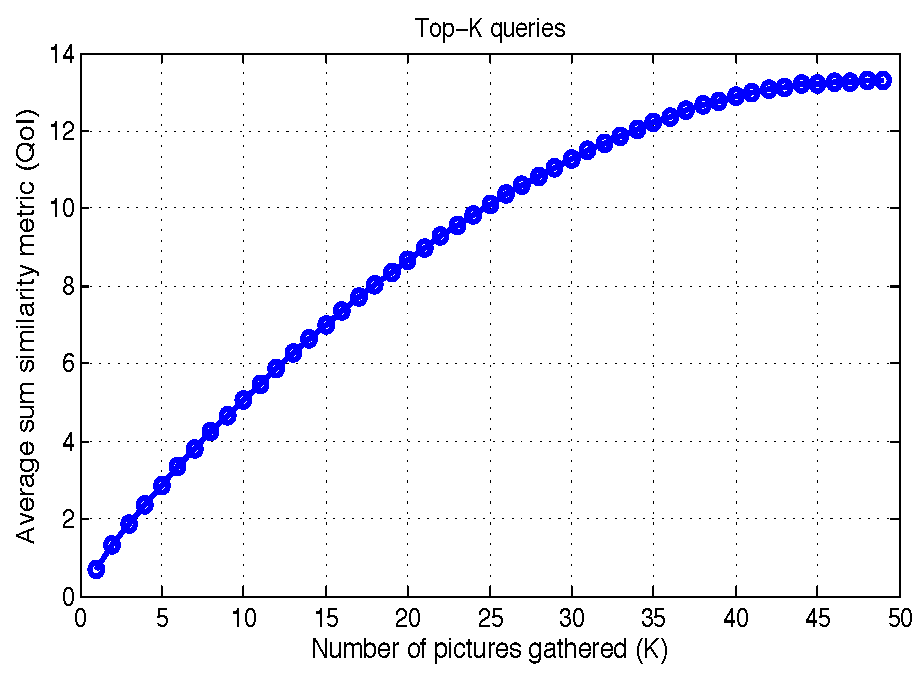
\includegraphics[scale=0.45]{figures/topkSumSimilarity.pdf}
    \caption{Sum Similartiy for Top-k Results of Varying $k$}
    \label{fig:spanAddDist}
\end{centering}
\end{figure}

%Spanner Cumulative Distance
\begin{figure} 
\begin{centering}
    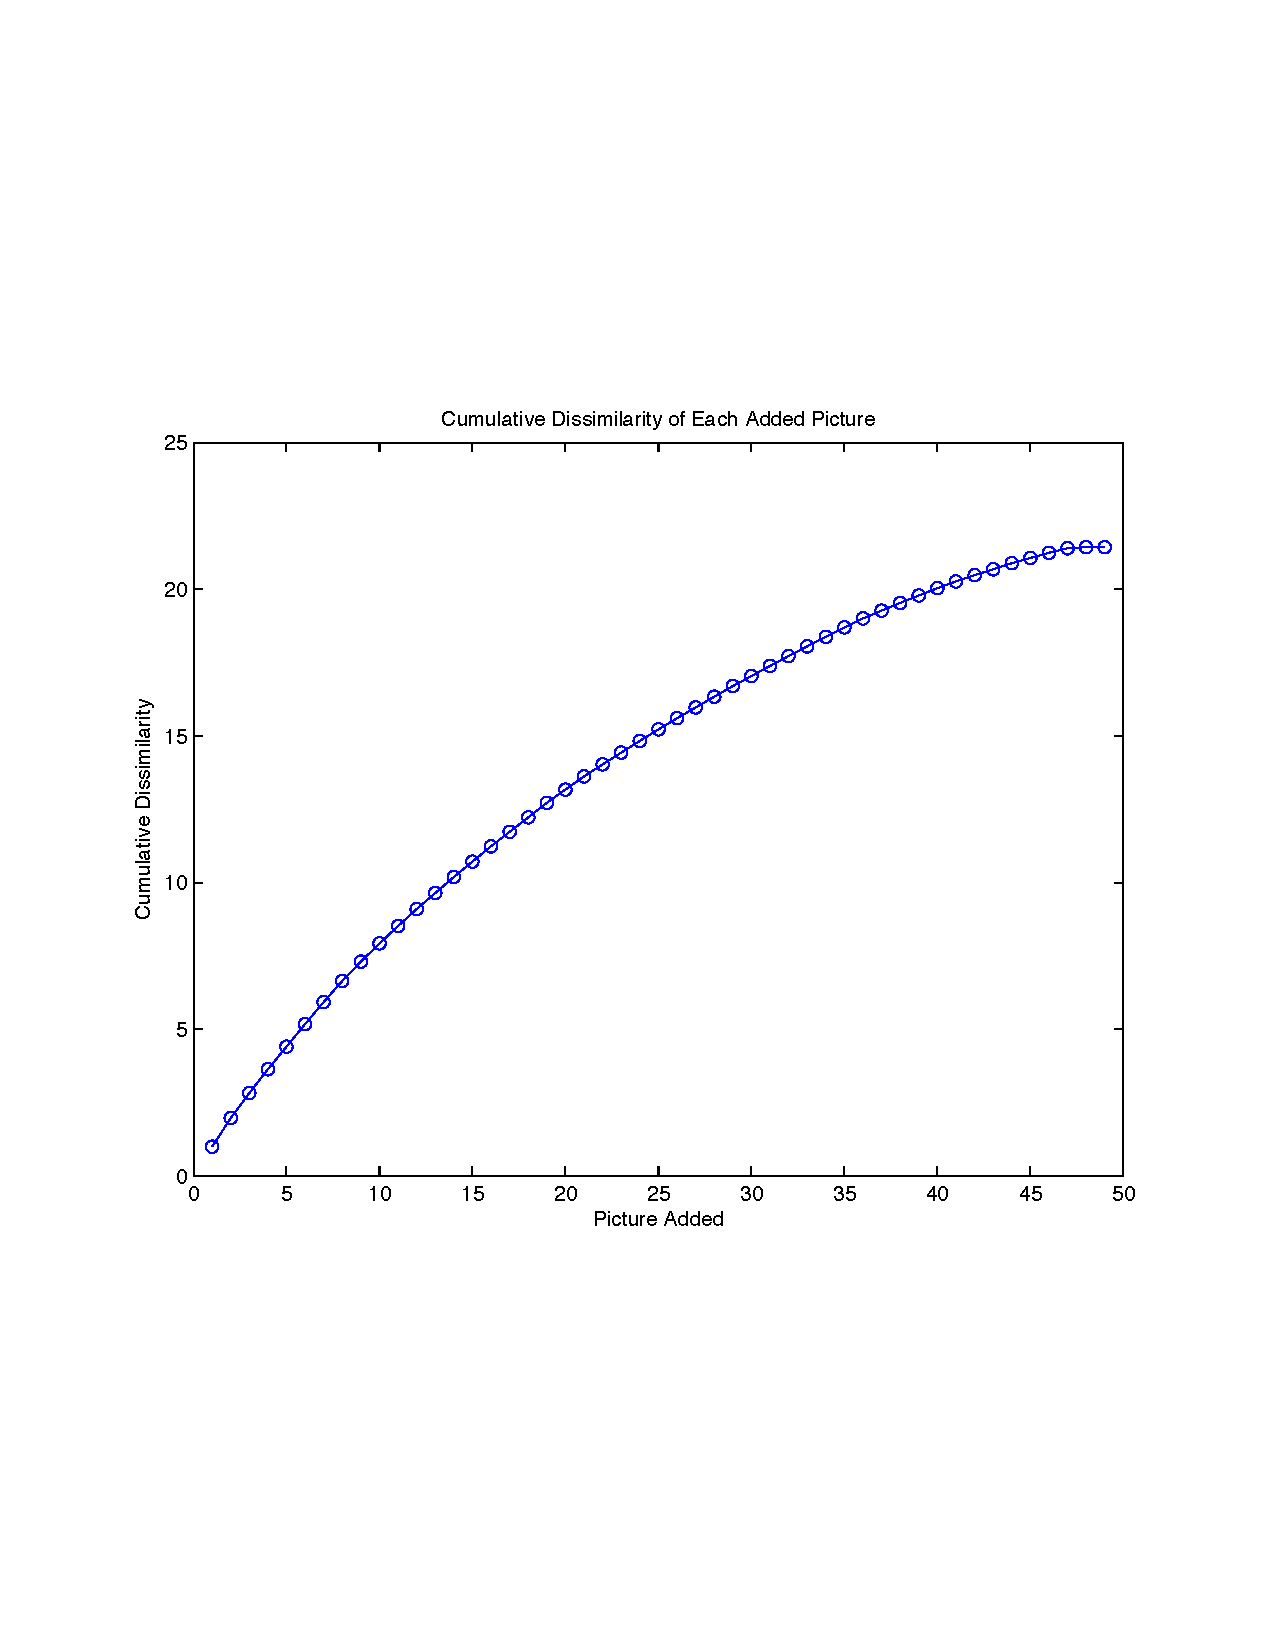
\includegraphics[scale=0.35]{figures/spannerCumulativeDist.pdf}
    \caption{Cumulative Distances for Spanners of Varying $k$ - Regular}
    \label{fig:spanCumDistReg}
\end{centering}
\end{figure}


%As for how we were planning to relate a notion of QoI which is increasing with more images;
%The Top_K query seems readily expandable for different K-you give a target image and as you collect more images you add more "similarity metrics"(which reduces with distances), but the spanner had some issues:
%If normalized among all distances, the average distance among elements reduces with more elements.
%On the other hand, if we simply add pairwise distances, it overcounts too many combinations (n choose 2)
%So, the latest possibility I had in mind was to consider an additive metric such that each introduced picture brings increases the metric proportion to either the avg distance to existing elements, or minimum/maximum of all distances to the existing elements. 
%Given the definition of "spanner", which is "Spanner maximizes the minimum dissimilarity between all pairs", what  I had in mind was perhaps to consider an additive metric such that each introduced picture increases the metric proportion to the minimum of all distances to the existing elements. Or, since the whole set of selected pictures might change with different 
%K, probably the best metric is:
%
%For a spanner of K pictures: Total "quality/diversity metric" = \sum_{i=1 to K} min_{j in K-i} (distance_i, j)
%
%that is, we run the spanner, find K pictures. For each picture we have a minimum dissimilartity/distance to rest of the pictures. Than, we add these minimum dissimilarities over all pictures. 
%I think the case where the extra metric added is in proportion to the average distances should decrease for each new added picture, so we should have a increasing concave type function.

%the graph is generated as follows: 
%given a timeliness T and dissimilarity(D)/similarity(S) requirement, we find how many nodes the network can scale up to, say N, by the scalability analysis formulas.
%Then we look at how many images are required for attaining D/S, say K(this comes from the CEDD based MATLAB analysis). With the assumption that each node has one image, this essentially implies a lower bound on the required network size in terms of number of nodes to attain D/S.
%If N<K, the network cant actually scale large enough to provide the similarity/dissimilarity, so it is not "scalably feasible".
%so this graph is obtained as follows; for each T, identify the largest D/S such that N>=K still holds.